\documentclass[12pt, letter]{exam}
\usepackage{enumerate}
%\usepackage[hmargin=2.0cm,vmargin=1cm]{geometry}
\usepackage[utf8]{inputenc}
\usepackage[spanish]{babel}
\usepackage{graphicx}
\usepackage{float}
\usepackage{cite}
\usepackage{natbib}
\usepackage{hyperref}
\usepackage{mdframed}
\mdfdefinestyle{mystyle}{leftmargin=1cm,rightmargin=1cm,linecolor=red}


\usepackage{upquote,textcomp}
\newcommand\upquote[1]{\textquotesingle#1\textquotesingle}
\date{}

\title{\begin{LARGE}
{Taller 3 Herramientas Computacionales: \LaTeX - Tablas, Figuras y Bibliograf\'ia}
\end{LARGE}}

\begin{document}

\maketitle


Esta tarea se debe entregar antes de las 2:00 pm del lunes 25 de agosto, se debe subir al SICUA un solo archivo comprimido que contenga en su interior lo siguiente: \verb'giro.sh', \verb'imagenes.tex' y \verb'referencias.tex'. Favor nombrar el archivo comprimido de acuerdo al formato \verb'NombreApellido_HW3.tar.gz'\\

\begin{questions}

\question (Tablas) En el archivo giro.csv se encuentra la informaci\'on de los tiempos de cada corredor del Giro de Italia de las primeras seis etapas.
Hacer un script que pase el archivo \verb"giro.csv" a formato \verb"giro.tex", y que además compile y genere un archivo \verb"tabla.pdf"; para
esto hacer uso del comando \verb+sed+ que sirve para hacer reemplazos en archivos de texto, tener en cuenta lo siguiente:

\begin{itemize}
\item \verb"sed 's/símbolo a quitar/símbolo a insertar/g'" \\
Toma el archivo de entrada y lo imprime con todas las ocurrencias del símbolo a quitar reemplazadas con el símbolo a insertar, los caracteres \verb+\+ y \verb+&+ son especiales y deben usarse como se explica más adelante.
\item \verb"sed 's/$/final/g'" \\
Toma el archivo de entrada y pone al final de cada línea el texto ``final''.
\item \verb"sed 's/^/inicio/g'" \\
Toma el archivo de entrada y pone al inicio de cada línea el texto ``inicio''.
\item Si quiere usar el caracter \verb+\+ en \verb+sed+ como parte de un texto tiene que ponerlo de la forma \verb+\\+, por ejemplo, si al final de cada línea quisiera poner \verb+\final+, debería invocar \verb+sed+ de la siguiente forma \verb+sed 's/$/\\final/g'+
\item El caracter \verb+&+ también es un caracter especial en \verb+sed+, siendo así tiene que ponerse de la forma \verb+\&+.
\item La coma \verb+,+  no es un caracter especial, es decir que si quisieran reemplazarse todas las comas con otro caracter se utilizaría el comando \\ \verb+sed 's/,/símbolo a insertar/g'+.
\end{itemize}
Asegúrese de entender el funcionamiento de \verb+sed+ antes de intentar resolver este ejercicio.
\newpage
\question (Imágenes) Hacer un archivo \verb"imagenes.tex" que reproduzca lo que se muestra abajo, en la parte donde se hace referencia a la figura (fig.\ 1) no vale escribir literalmente ``fig.\ 1'', tiene que usar el comando \verb+\ref+. 

\DeclareGraphicsExtensions{.pdf,.png,.jpg}

\begin{mdframed}[style=mystyle]
\vspace{0.5cm}
En la fig.\ \ref{fig:ISS} se muestra la \textit{Estación Espacial Internacional} atravesando la Luna.

\begin{figure}[H]
\centering
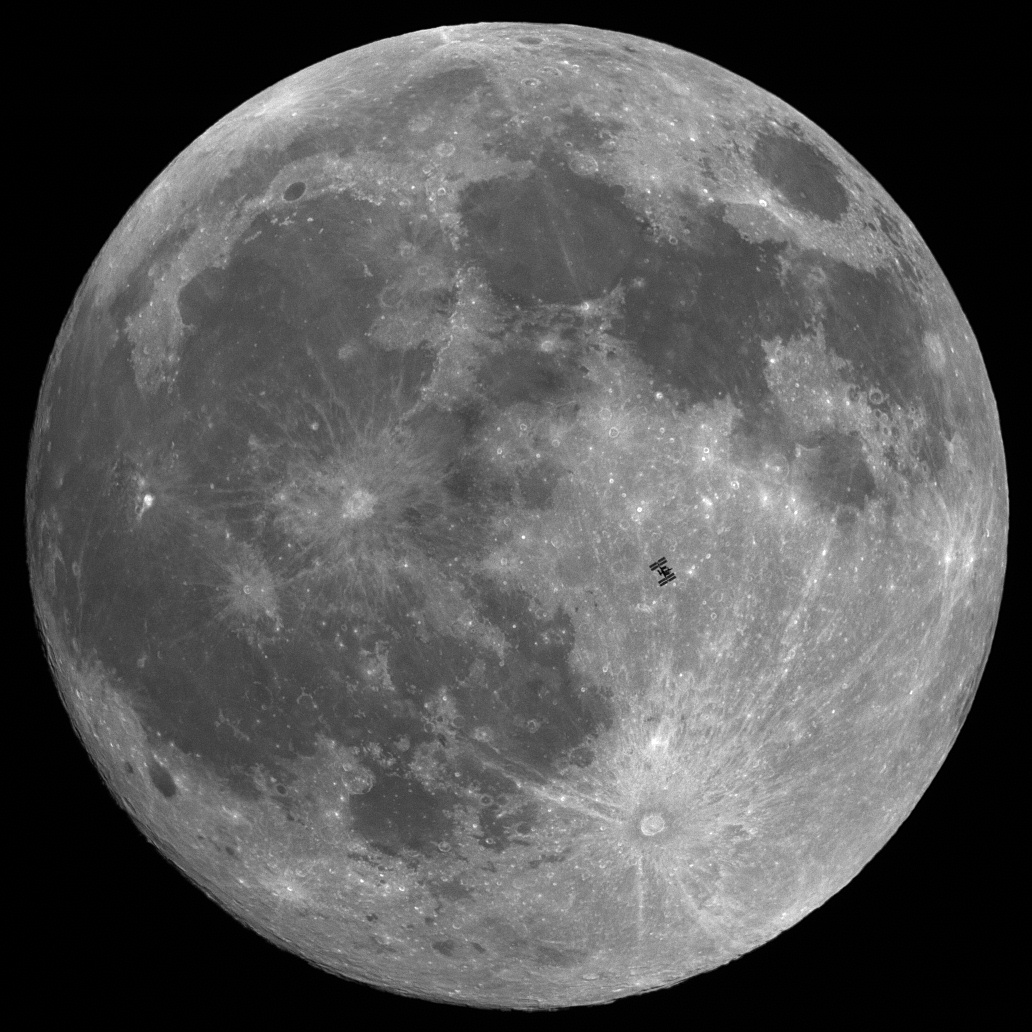
\includegraphics[scale=0.4]{ISS_moon}
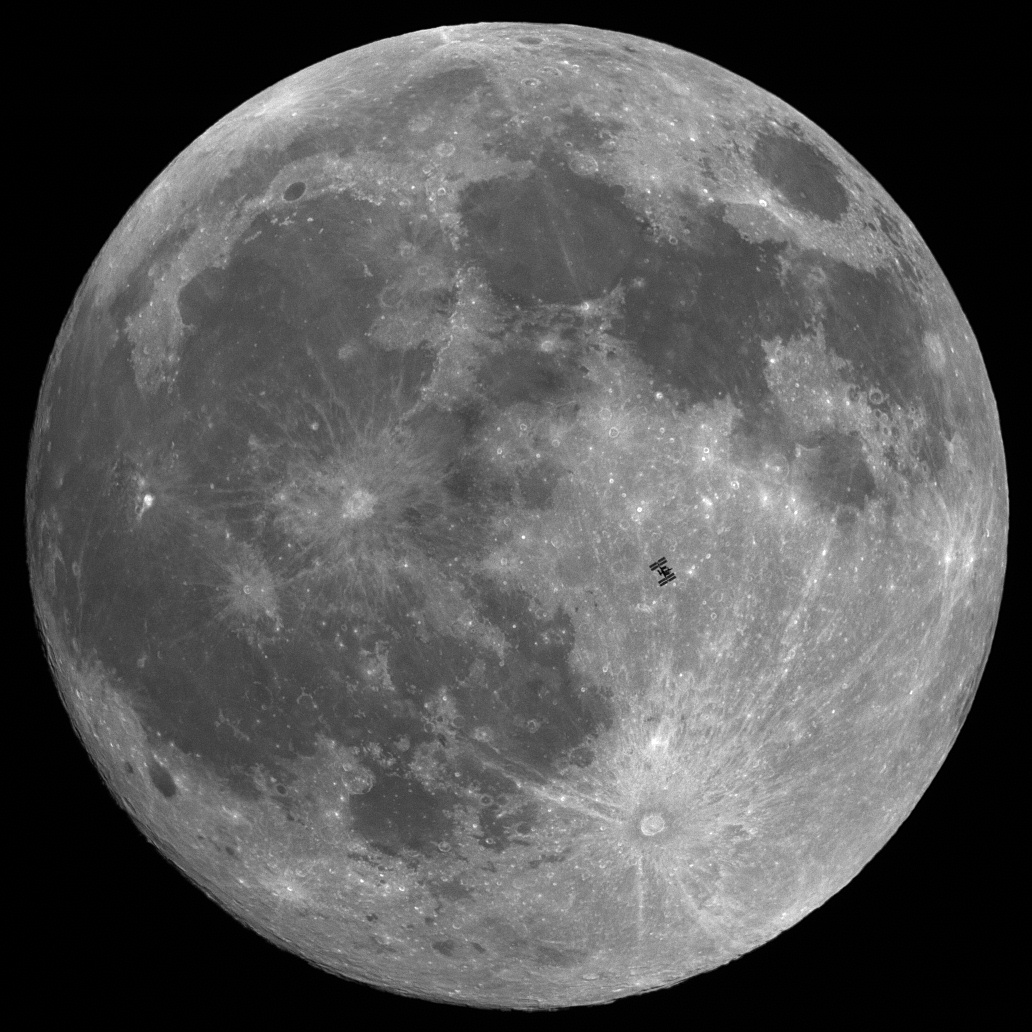
\includegraphics[scale=0.2]{ISS_moon}
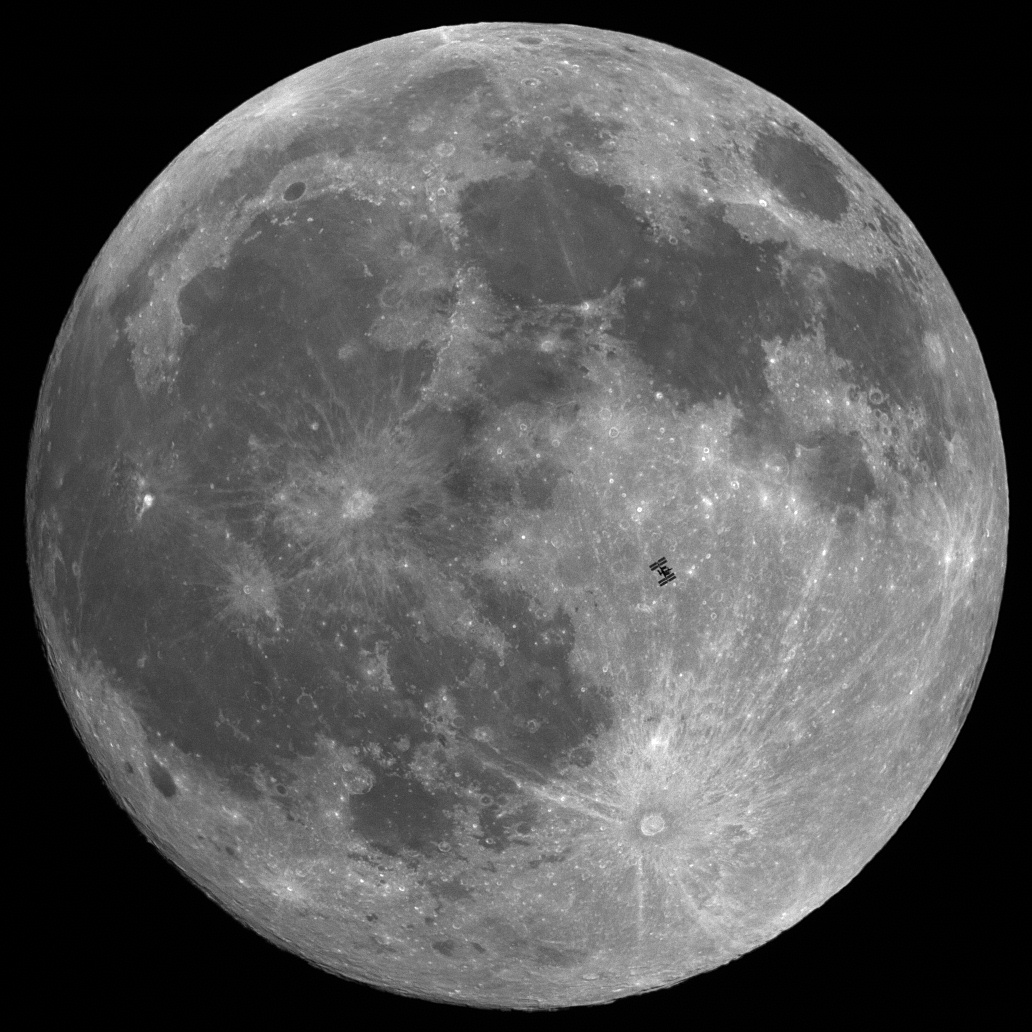
\includegraphics[scale=0.2, angle=45]{ISS_moon}
\caption{International Space Station (ISS), Moon transit.}
\label{fig:ISS}
\end{figure}
\end{mdframed}

\question{(Bibliograf\'ia)} En el archivo \verb"referencias.bib" se encuentra la bibliografía de este documento. Cree el archivo \verb+referencias.tex+ donde se reproduzca lo de abajo luego de invocar \verb+pdflatex - bibtex - pdflatex - pdflatex+. En el archivo de \LaTeX \,asegúrese de utilizar los comandos \verb+\bibliography, \bibliographystyle+ y \verb+\cite+.

\begin{mdframed}[style=mystyle]
\vspace{0.2cm}
En \citep{website:Latex-Graphics} pueden leer  sobre el manejo de gráficas en latex, en \citep{website:Latex-Figures} sobre el manejo de figuras, en \citep{website:Latex-Tables} sobre el manejo de tablas
y en \citep{website:Latex-Bibliography} sobre el manejo de la bibliografía. 

Si encuentran referencias adicionales que fueron útiles para hacer la tarea por favor colóquenlas y pongan las referencias.
 
\bibliography{references}{}
\bibliographystyle{plain}
\end{mdframed}

\end{questions}

\end{document}
